\section{Implementação}

\begin{frame}[fragile]{Construtor da UFDS}

    \begin{itemize}
        \item Considere que cada um dos $N$ conjuntos a serem representados na UFDS sejam
            identificados pelos inteiros de 1 a $N$

        \item A UFDS tem dois vetores membros: $size$ e $ps$

        \item $size[i]$ corresponde ao número de nós da árvore que tem $i$ como raiz

        \item $ps[i]$ é o pai de $i$ na árvore que ele está contido

        \item Como inicialmente todos os conjuntos são disjuntos, temos $size[i] = 1$
            e $ps[i] = i$, para $i = 1, 2, \ldots, N$

        \item Observe que, ao contrário da convenção das árvores em computação, o pai da raiz
            é ele próprio, o que simplifica a implementação

    \end{itemize}

\end{frame}

\begin{frame}[fragile]{Implementação do construtor da UFDS}
    \inputsnippet{cpp}{1}{17}{codes/ufds.h}
\end{frame}

\begin{frame}[fragile]{Identificação dos representantes}

    \begin{itemize}
        \item O método \code{cpp}{find_set(x)} retorna o representante (raiz) da árvore onde 
            $x$ se encontra

        \item Para isso, basta seguir a cadeia de pais, até localizar um nó cujo pai é ele
            mesmo

        \item Se a união for baseada no tamanho das árvores, o tamanho de cada árvore tende a
            $O(\log N)$, de modo que este método também tem complexidade $O(\log N)$

        \item O método \code{cpp}{same_set(x, y)} retorna verdadeiro se $x$ e $y$ pertencem a 
            mesma árvore, ou falso, caso contrário

        \item A implementação é simples: basta confrontar os representantes de cada conjunto
    \end{itemize}

\end{frame}

\begin{frame}[fragile]{Implementação da identificação de representantes}
    \inputsnippet{cpp}{19}{27}{codes/ufds.h}
\end{frame}

\begin{frame}[fragile]{União de conjunto disjuntos}

    \begin{itemize}
        \item O método \code{cpp}{union_set(x, y)} une as árvores onde $x$ e $y$ estão localizados

        \item Se $x$ e $y$ já estão na mesma árvore, nada deve ser feito

        \item Caso contrário considere, sem perda de generalidade, que a árvore que o número de nós da árvore contém $x$ seja
            maior ou igual que o número de nós da árvore que contém $y$

        \item Neste caso, a raiz da árvore de $x$ passa ser o pai da raiz da árvore de $y$

        \item Como ambas raízes devem ser localizadas previamente, a complexidade deste método
            também é $O(\log N)$
            
    \end{itemize}

\end{frame}

\begin{frame}[fragile]{Visualização da união de árvores}

    \begin{figure}
        \centering

        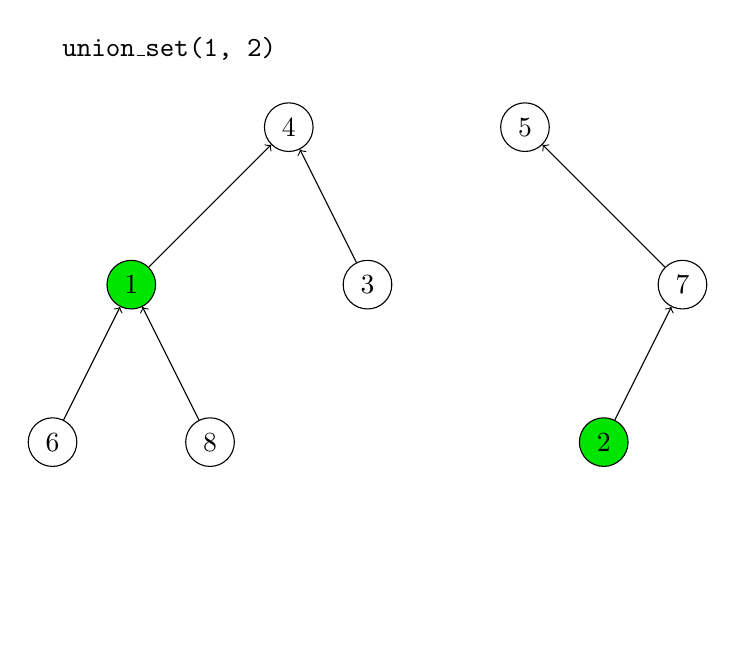
\begin{tikzpicture}
            \node[anchor=west] at (0, 6) { \tt union\_set(1, 2) };

            \node[draw,circle] (A) at (3, 5) { 4 };
            \node[draw,circle,fill=green!90!black] (B) at (1, 3) { 1 };
            \node[draw,circle] (C) at (4, 3) { 3 };
            \node[draw,circle] (D) at (0, 1) { 6 };
            \node[draw,circle] (E) at (2, 1) { 8 };

            \node[draw,circle] (F) at (6, 5) { 5 };
            \node[draw,circle] (G) at (8, 3) { 7 };
            \node[draw,circle,fill=green!90!black] (H) at (7, 1) { 2 };
            \node[draw,circle,opacity=0] (I) at (7, -1) { 2 };

            \draw[->] (B) edge (A);
            \draw[->] (C) edge (A);
            \draw[->] (D) edge (B);
            \draw[->] (E) edge (B);

            \draw[->] (G) edge (F);
            \draw[->] (H) edge (G);

        \end{tikzpicture}

    \end{figure}

\end{frame}

\begin{frame}[fragile]{Visualização da união de árvores}

    \begin{figure}
        \centering

        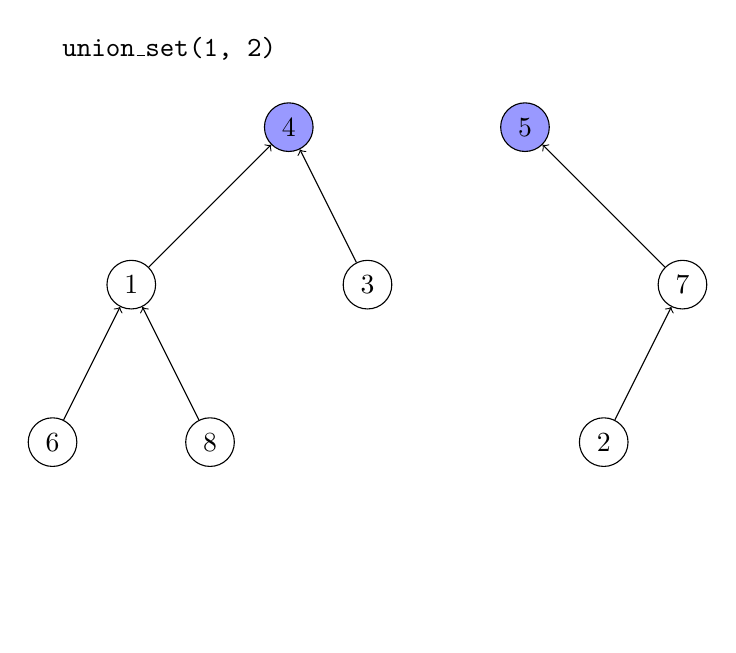
\begin{tikzpicture}
            \node[anchor=west] at (0, 6) { \tt union\_set(1, 2) };

            \node[draw,circle,fill=blue!40] (A) at (3, 5) { 4 };
            \node[draw,circle] (B) at (1, 3) { 1 };
            \node[draw,circle] (C) at (4, 3) { 3 };
            \node[draw,circle] (D) at (0, 1) { 6 };
            \node[draw,circle] (E) at (2, 1) { 8 };

            \node[draw,circle,fill=blue!40] (F) at (6, 5) { 5 };
            \node[draw,circle] (G) at (8, 3) { 7 };
            \node[draw,circle] (H) at (7, 1) { 2 };
            \node[draw,circle,opacity=0] (I) at (7, -1) { 2 };

            \draw[->] (B) edge (A);
            \draw[->] (C) edge (A);
            \draw[->] (D) edge (B);
            \draw[->] (E) edge (B);

            \draw[->] (G) edge (F);
            \draw[->] (H) edge (G);

        \end{tikzpicture}

    \end{figure}

\end{frame}

\begin{frame}[fragile]{Visualização da união de árvores}

    \begin{figure}
        \centering

        \begin{tikzpicture}
            \node[anchor=west] at (0, 6) { \tt union\_set(1, 2) };

            \node[draw,circle] (A) at (3, 5) { 4 };
            \node[draw,circle] (B) at (1, 3) { 1 };
            \node[draw,circle] (C) at (4, 3) { 3 };
            \node[draw,circle] (D) at (0, 1) { 6 };
            \node[draw,circle] (E) at (2, 1) { 8 };

            \node[draw,circle] (F) at (6, 3) { 5 };
            \node[draw,circle] (G) at (8, 1) { 7 };
            \node[draw,circle] (H) at (7, -1) { 2 };
            \node[draw,circle,opacity=0] (I) at (7, -1) { 2 };

            \draw[->] (B) edge (A);
            \draw[->] (C) edge (A);
            \draw[->] (D) edge (B);
            \draw[->] (E) edge (B);

            \draw[->] (F) edge (A);
            \draw[->] (G) edge (F);
            \draw[->] (H) edge (G);

        \end{tikzpicture}

    \end{figure}

\end{frame}




\begin{frame}[fragile]{Implementação da união de conjuntos disjuntos}
    \inputsnippet{cpp}{29}{49}{codes/ufds.h}
\end{frame}
